\documentclass{article}
\usepackage{amsmath}
\usepackage{tikz}
\usetikzlibrary{bayesnet}
\begin{document}
\def\blw{\boldsymbol{w}}
\def\blf{\boldsymbol{f}}
\def\blphi{\boldsymbol{\phi}}
\renewcommand\phi\varphi


\textbf{Notation:}
\begin{table}[h]
\begin{tabular}{ll}
$N$                   & number of VSO triples (indexed by $i$)                      \\
$F$                   & number of frames (indexed by $f$)                       \\
$V$                   & vocabulary size (indexed by $w$)\footnotemark\\
$\blf$                   & the sequence of frames (one for each triple)        \\
$f_i$                 & $1\leq f_i\leq F$ is the frame assigned to the $i$th triple      \\
$\blw$           & the sequence of VSO triples (this is our data)                               \\
$ w_i$            & $i$th triple                                            \\
$w_i^{(a)}$           & the word with syntactic role $a$ ($a\in\{s,v,o\}$) in the $i$th triple \\
$\blphi$          & sequence probability distributions characterizing frames    \\
$\phi_f$          & probability distributions for frame $f$                  \\
$\phi_f^{(a)}$        & probability distribution for syntactic role $a$ in frame $f$ \\
$C(w,f,a)$          & number of times that $w$ appears in position $a$ in triples assigned to frame $f$\\
\end{tabular}
\end{table}
\footnotetext{We may want to have a separate vocabulary for each syntactic role
($V^{(s)},V^{(v)},V^{(o)}$)... for now lump them all together and make use of 0 counts.}

The generative story for model 0 is

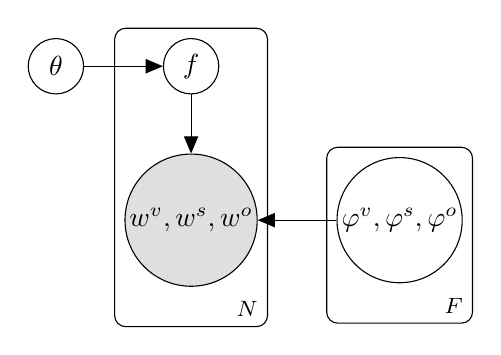
\begin{tikzpicture}
  % Nodes
  \node[obs] (datapoint) {$w^v,w^s,w^o$} ; %
  \node[latent, above=0.75cm of datapoint] (F) {$f$} ; %
  \node[latent, left=of F] (theta) {$\theta$}; %
  \node[latent, right=of datapoint] (phi) {$\varphi^v,\varphi^s,\varphi^o$}; %
  \edge {theta} {F} ; %
  \edge {F} {datapoint}
  \edge {phi} {datapoint} ; %
  \plate {tuples} {(F) (datapoint) } {$N$}; %
  \plate {} {(phi)} {$F$} ; %
\end{tikzpicture}


\[
P(\blf,\blw,\blphi|\theta,\beta)
= P(\blf|\theta)P(\blw|\blphi)P(\blphi|\beta)
\]

\begin{align*}
p(f|\theta)      =& \prod_{i=1}^{N}\theta(f_i)\\
p(w|\blphi,\blf) =& \prod_{i=1}^N\prod_{a}^{\{v,s,o\}}\phi_{f_i}^a(w_i^a)\\
                 =& \prod_{f=1}^{F}\prod_{w=1}^{V}\prod_{a}^{\{s,v,o\}}\phi_f^a(w)^{C(w,f,a)}\\
p(\phi|\beta)    =& (\frac{3}{B(\beta)})^K\prod_{f=1}^{F}\prod_{w=1}^{V}\prod_{a}^{\{s,v,o\}}\phi_f^a(w)
\end{align*}

So we have...

\begin{align*}
\prod_{i=1}^{N}\theta(f_i) \times
\prod_{f=1}^{F}\prod_{w=1}^{V}\prod_{a}^{\{s,v,o\}}\phi_f^a(w)^{C(w,f,a)} \times
& (\frac{3}{B(\beta)})^K\prod_{f=1}^{F}\prod_{w=1}^{V}\prod_{a}^{\{s,v,o\}}\phi_f^a(w)\\
= \prod_{i=1}^{N}\theta(f_i) \times
(\frac{3}{B(\beta)})^K
\prod_{f=1}^{F}\prod_{w=1}^{V}\prod_{a}^{\{s,v,o\}}\phi_f^a(w)^{(C(w,f,a) + 1)}
\end{align*}

\begin{align*}
p(\blf,\blw|\theta,\beta) =& \int p(\blf,\blw,\blphi|\theta,\beta) d\phi\\
=& 
\prod_{i=1}^{N}\theta(f_i) \times
\int\prod_{f=1}^{F}\prod_{w=1}^{V}\prod_{a}^{\{s,v,o\}}\phi_f^a(w)^{(C(w,f,a) + 1)}d\phi
\end{align*}


\end{document}
